\documentclass[../notes.tex]{subfiles}
\graphicspath{{\subfix{../img/}}}
\begin{document}

\section{System Identification \& Analysis}
Before we can understand how to control a system, we must first understand how that system changes in response to input. System identification is the process by which a mathematical model of the dynamical system can be constructed. Designing a controller is infinitely easier with such a model. 
\begin{emphasis}
    The system (excluding the controller) is referred to as the "plant".
\end{emphasis}

\subsection{Linear Regression}
\subsection{State-space Models}
State space models are a useful way to describe a system. A typical LTI system can be arranged as follows:
\begin{equation*}
    x(t) - \text{state} \quad y(t) - \text{output} \quad u(t) - \text{input}
\end{equation*}
\begin{align*}
    \dot{x}(t) &= Ax(t) + Bu(t) \\
    y(t) &= Cx(t) + Du(t)
\end{align*}
\begin{align*}
    A &\in \mathbb{R}^{n_x \times n_x} \quad \text{zero input dynamics matrix}\\
    B &\in \mathbb{R}^{n_x \times n_u} \quad \text{input matrix}\\
    C &\in \mathbb{R}^{n_y \times n_x} \quad \text{output matrix}\\
    D &\in \mathbb{R}^{n_y \times n_u} \quad \text{pass-through matrix}
\end{align*}


\subsection{Linear, Time-Invariant Systems (LTI)}

\subsubsection{Properties}
\begin{description}
    \item[Homogeneity] $\begin{cases*}
        x(t_0), u(t) \rightarrow y(t) \\
        \alpha x(t_0), \alpha u(t_0) \rightarrow \alpha y(t)
    \end{cases*}$
    \item[Additivity] $\begin{cases*}
        x_1(t_0), u_1(t) \rightarrow y_1(t) \\
        x_2(t_0), u_2(t) \rightarrow y_2(t)
    \end{cases*} \Rightarrow x_1(t_0) + x_2(t_0), u_1(t) + u_2(t) \rightarrow y_1(t) + y_2(t)$
    \item[Time Invariance] For the same input, the response at an time will be the same.
\end{description}

\subsubsection{Convolution}
The uniformity and superposition allows us to use the response to a known unput to comput the response to a generic input. Convolution is the mathematical operation  by which we generate the response to said generic input. It's only because of the time uniformity and superposition that convolution is useful and gets its own name (unlike other mathematical constructs). \\
In the time domain the definition is:
\begin{equation}
    y(t) = [h*u](t) = \int_{0}^{t}h(\tau)u(t-\tau)d\tau = \int_{0}^{t}h(t-\tau)u(\tau)d\tau
\end{equation}
Where h(t) is the impulse response of the LTI system impulse response is the response to a unit impulse $\delta(t)$.
\begin{equation}
    \delta(t) = \begin{cases}
        \infty, \text{ at } t=0 \\
        0 \text{ otherwise}
    \end{cases}
\end{equation}
Assuming zero initial conditions:
\begin{equation*}
    h(t) = Ce^{At}B + D\delta(t)
\end{equation*}
The impulse response is by definition a time domain concept, as it is defined as the time domain output of an LTI system to a unit time domain impulse in the input.
\paragraph{Visualization of Convolution}
The input can be interpreted as a sequence of impulses offset in time, each setting off its own impulse response that is scaled in magnitude by the magnitude of $u(t)$ at said time. The output can be understood as the sum of the resulting scaled and time shifted impulse responses. \\
For any initial condition the output $y(t)$ of an LTI system due to a sinusoidal input $u(t)$ will converge to a steady state output $y_{ss}(t)$ as $t\rightarrow\infty$, assuming a steady state output exists. The output will be a sinusoid of the same frequency as $u(t)$, with a different magnitude and phase shift. The magnitude and phase shift can be gleaned from the transfer function (specifically from the Bode plot).\\
Each block in a control diagram represents a convolution. Thus, we need a more intuitive way to perform the operation, which can be done in the frequency domain, which can be done with the Laplace transform.

\subsection{Linear, Time-Varying Systems (LTV)}
For an LTV system, the system is time-varying because at least one of the four system matrices changes with time, not because $x,y,u$ change with time! The primary shortcoming of LTV systems is their dependence on the initial time. An input and initial condition might have different responses over different time intervals. We cannot guarantee homogeneity and additivity over shifted time intervals.
\begin{align*}
    \dot{x}(t) &= A(t)x(t) + B(t)u(t) \\
    y(t) &= C(t)x(t) + D(t)u(t)
\end{align*}
\begin{equation*}
    A(t) \in \mathbb{R}^{n_x \times n_x} \quad
    B(t) \in \mathbb{R}^{n_x \times n_u} \quad
    C(t) \in \mathbb{R}^{n_y \times n_x} \quad
    D(t) \in \mathbb{R}^{n_y \times n_u} 
\end{equation*}
\subsubsection{Properties}
\begin{description}
    \item[Homogeneity] $\begin{cases*}
        x(t_0), u(t) \rightarrow y(t) \\
        \alpha x(t_0), \alpha u(t_0) \rightarrow \alpha y(t)
    \end{cases*}$
    \item[Additivity] $\begin{cases*}
        x_1(t_0), u_1(t) \rightarrow y_1(t) \\
        x_2(t_0), u_2(t) \rightarrow y_2(t)
    \end{cases*} \Rightarrow x_1(t_0) + x_2(t_0), u_1(t) + u_2(t) \rightarrow y_1(t) + y_2(t)$
\end{description}
Together, these two properties are called \underline{superposition}. These properties do not hold under time shifts, however.
\paragraph{State Transition Matrix}
Governs zero-input dynamics.
\begin{equation*}
    \Phi_A(t_0,t_0) = I_{n_x \times n_x}, \quad \dot{\Phi}_A(t_0,t_0) = A(t)\Phi_A(t_0,t_0)
\end{equation*}
\subsection{Modal Analysis}
Eigenvalues (\underline{\ref{sec:eig}}) are critical for understanding how a system reacts to input. A mode of a system is the time response associated with either a simple eigenvalue and associated eigenvector, or a complex conjugate pair of eigenvalues + eigenvectors. \\
Maximum number of modes is $n_x$, and minimum is $n_x / 2$ (which is if all eigenvalues are complex conjugate pairs.)
\begin{equation*}
    \dot{x}(t) = Ax(t)
\end{equation*}
If we define the initial conditions as:
\begin{align*}
    x(0) &= v_i \text{ where $v_i$ is an eigenvector of }A \\
    \dot{x}(0) &= Ax(0) = Av_i = \lambda_i v_i
\end{align*}
Since $\lambda$ is a scalar, this equation implies the state of the system will evolve parallel to $v_i$. This means that $\dot{x}(t)$ will always remain aligned with $v_i$, and $x(t)$ will never come out of alignment.
\paragraph{Observations}
\begin{itemize}
    \item The real part of the eigenvalue $\lambda_i$ dictates the exponential growth of decay of $x_{mj}(t)$.
    \item The imaginary part of eigenvalue $\lambda_i$ dictates the frequency with which $x_{mj}(t)$ oscillates.
    \item The eigenvector $v_i$ encodes the relative phase and magnitude of each state in $x(t)$. The phase information is encoded by the relative phase of the complex elements of the vector $v_i$.
    \item The scalar $\alpha_0$ determines theh initial scaling and phase shift of all the states in $x(t)$.
\end{itemize}
\begin{equation*}
    X_{mj}(t) = \alpha_0 v_i e^{\lambda_i t} = \alpha_0 v_i e^{\text{Re}(\lambda_i)t}[\cos(\text{Im}(\lambda_i)t) + j\sin(\text{Im}(\lambda_i)t)]
\end{equation*}
Any zero input motion that a given LTI system can exhibit can be expressed as a superposition of the system modes.

\paragraph{Example: Conventional Aircraft Modes}
\begin{description}
    \item[Phugoid]
    \item[Dutch Roll]
    \item[Subsidence]   
\end{description}

\paragraph{Example: System Modes}
Take the following 2D mass-spring-damper system:
\begin{figure}[H]
    \centering
    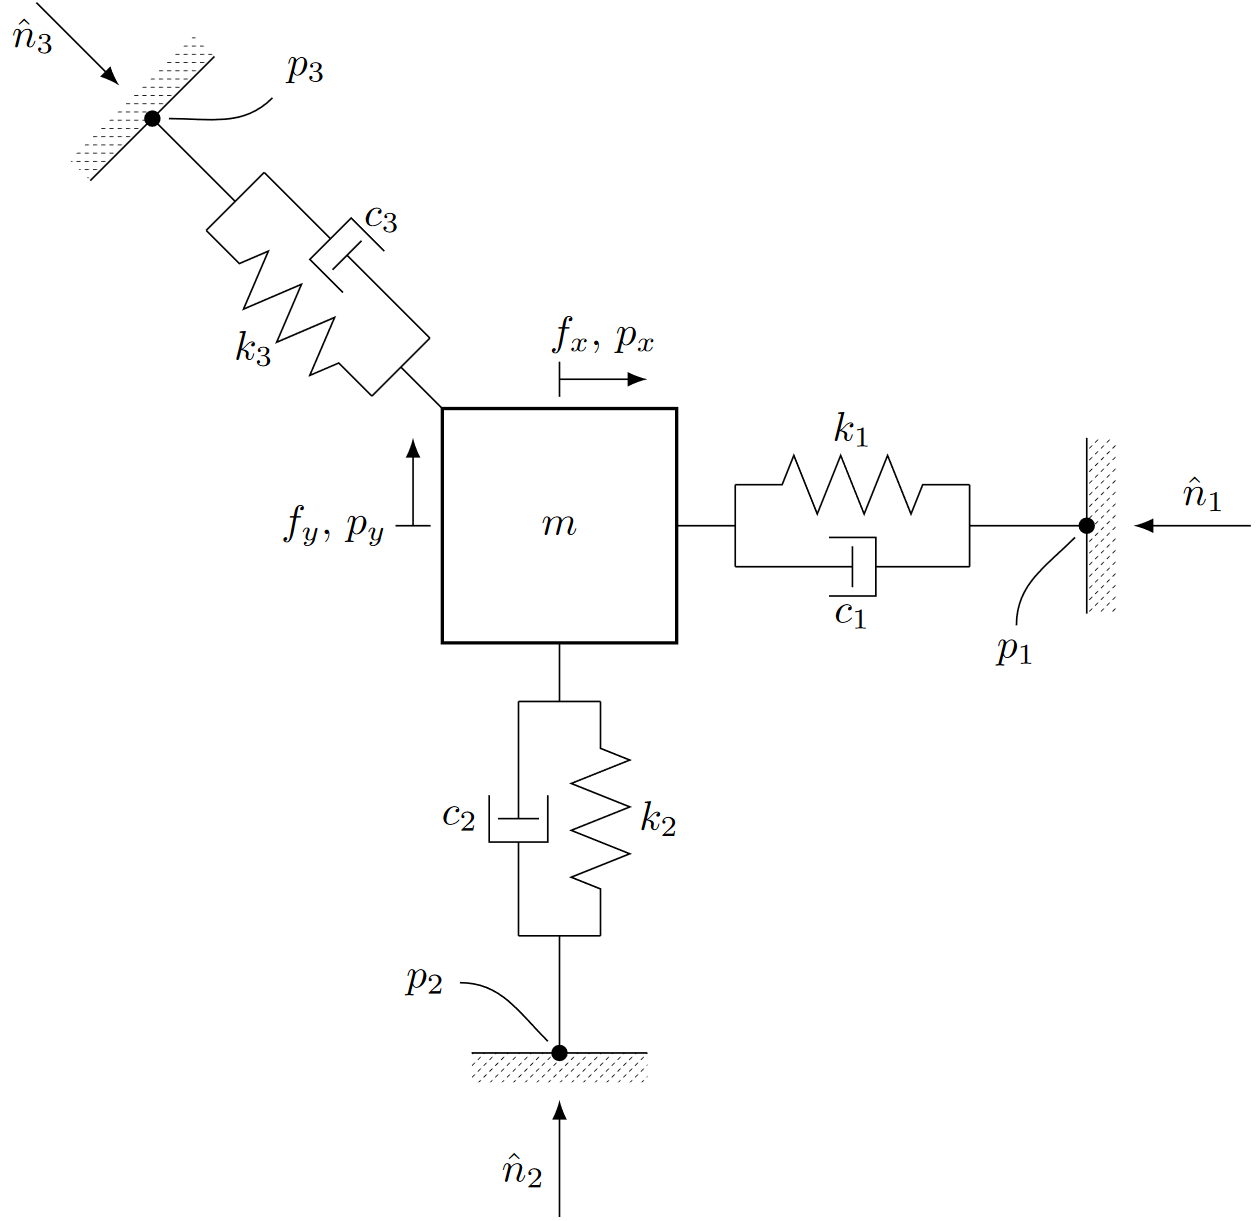
\includegraphics[width=1\linewidth]{2dMSD.png}
    \caption{2D Nonlinear Mass-Spring-Damper System}
    \label{fig:2dMSD}
\end{figure}
We can define the state, control input, and desired output vectors as follows:

\begin{equation*} 
  x(t) =
  \begin{bmatrix}
  p_{x}\\ 
  p_{y}\\ 
  \dot{p_x}(t)\\ 
  \dot{p_y}(t) 
  \end{bmatrix},
\quad
  u(t) =
  \begin{bmatrix}
  f_{x}\\ 
  f_{y}
  \end{bmatrix},
\quad
  y(t) =
  \begin{bmatrix}
  p_{x}\\ 
  p_{y}
  \end{bmatrix}
\end{equation*}

For this system, gravity can be neglected. We can define variables as follows: $\delta_i$ is the displacement of each mass/damper pair, $\dot{\delta}_i$, is the rate of displacement of each mass/damper pair, $\hat{n}_i$ is the unit vector pointing from the attachment point of each mass/damper pair towards the position of the mass. The variables $k_i$ and $c_i$ are the spring and damper constants respectively, where $i$ represents each mass/damper grouping. 

In order to find the function describing the dynamics of the system, the state vector is differentiated, because $\dot{x}(t) = f(x(t), u(t))$. The second derivative of the position of the mass, $\Ddot{p}$, can be found using Newton's Laws of Motion, as seen in Eq. \ref{eq:xdot}.

\begin{equation} \label{eq:xdot}
    \dot{x}(t) = 
    \begin{bmatrix}
        \dot{p}_{x}(t) \\
        \dot{p}_{y}(t) \\
        \ddot{p}_{x}(t) \\
        \ddot{p}_{y}(t) \\
    \end{bmatrix}
    \Rightarrow
    \begin{bmatrix}
        \dot{p}_{x}(t) \\
        \dot{p}_{y}(t) \\
        \sum [k_i \cdot \delta_i \cdot \hat{n}_{x, i}] + \sum [c_i \cdot \dot{\delta}_i \cdot \hat{n}_{x, i}] + f_x \\
        \sum [k_i \cdot \delta_i \cdot \hat{n}_{y, i}] + \sum [c_i \cdot \dot{\delta}_i \cdot \hat{n}_{y, i}] + f_y \\
    \end{bmatrix}
\end{equation}

Next, the equations of the system can be derived by linearizing about the equilibrium point, represented by $\Bar{x}(t)$ and $\Bar{y}(t)$. The linearization is done by holding one variable constant about the equilibrium point while the derivative with respect to the other is computed. The system matrices calculated (numerical Jacobian) from the initial system variables given are:

\begin{equation*} 
  A =
  \begin{bmatrix}
    0 &0 &1 &0\\ 
    0 &0 &0 &1\\
    -2.5 &1.5 &0 &0\\
    1.5 &-3.5 &0 &0
  \end{bmatrix},
\quad
  B =
    \begin{bmatrix}
        0 &0 \\ 
        0 &0 \\
        1 &0 \\
        0 &1
    \end{bmatrix},
\quad
  C =
  \begin{bmatrix}
  1 &0 &0 &0 \\
  0 &1 &0 &0
  \end{bmatrix},
  \quad
  D =
  \begin{bmatrix}
  0 &0\\ 
  0 &0
  \end{bmatrix}
\end{equation*}

MATLAB's built in \verb|eig()| function can be used to find the eigenvalues and corresponding eigenvectors. The eigenvalues and their corresponding eigenvectors are found below. Each row in the eigenvalue vector corresponds to the same indexed column in the eigenvector matrix.

\begin{equation*}
    \lambda = 
    \begin{bmatrix}
        -0 + 2.1404i \\
        -0 - 2.1404i \\ 
         0 + 1.1912i \\
         0 - 1.1912i
    \end{bmatrix},
    \quad
    v = 
    \begin{bmatrix}
        0 + 0.2475i  &0 - 0.2475i   &0 - 0.5216i   &0 + 0.5216i \\
        0 - 0.3434i  &0 + 0.3434i   &0 - 0.3760i   &0 + 0.3760i \\ 
        -0.5297 - 0i  &-0.5297 + 0i   &0.6213 + 0i   &0.6213 + 0i \\ 
         0.7350 + 0i  & 0.7350 + 0i   &0.4478 + 0i   &0.4478 - 0i
    \end{bmatrix}
\end{equation*}

The A matrix has two complex conjugate pairs of eigenvectors, meaning that the system has two modes. The modes are found by taking the real part of the complex eigenvectors and plugging them in as the initial state. The first two eigenvectors correspond to the direction seen in Fig. \ref{fig:mode1}, and the second two correspond to Fig. \ref{fig:mode2}. Both modes oscillate, although the first mode oscillates faster. Neither exponentially grows for two reasons: there is no forcing input applied, and the absence of damping results in a purely imaginary eigenvalue, which means motion is purely oscillatory with no gain. Neither exponentially decays for the same reason. The relationship between the modes and the damping coefficients is such that when the system is undamped, it is in a state of pure oscillation, and thus the eigenvalues are purely imaginary. Adding a damping coefficient adds a real component to the eigenvalues, which represents the damping effect. Moreover, the damped natural frequency will be less than that of an undamped system.

\begin{figure}[H]
    \centering
    \begin{subfigure}{.5\textwidth}
        \centering
        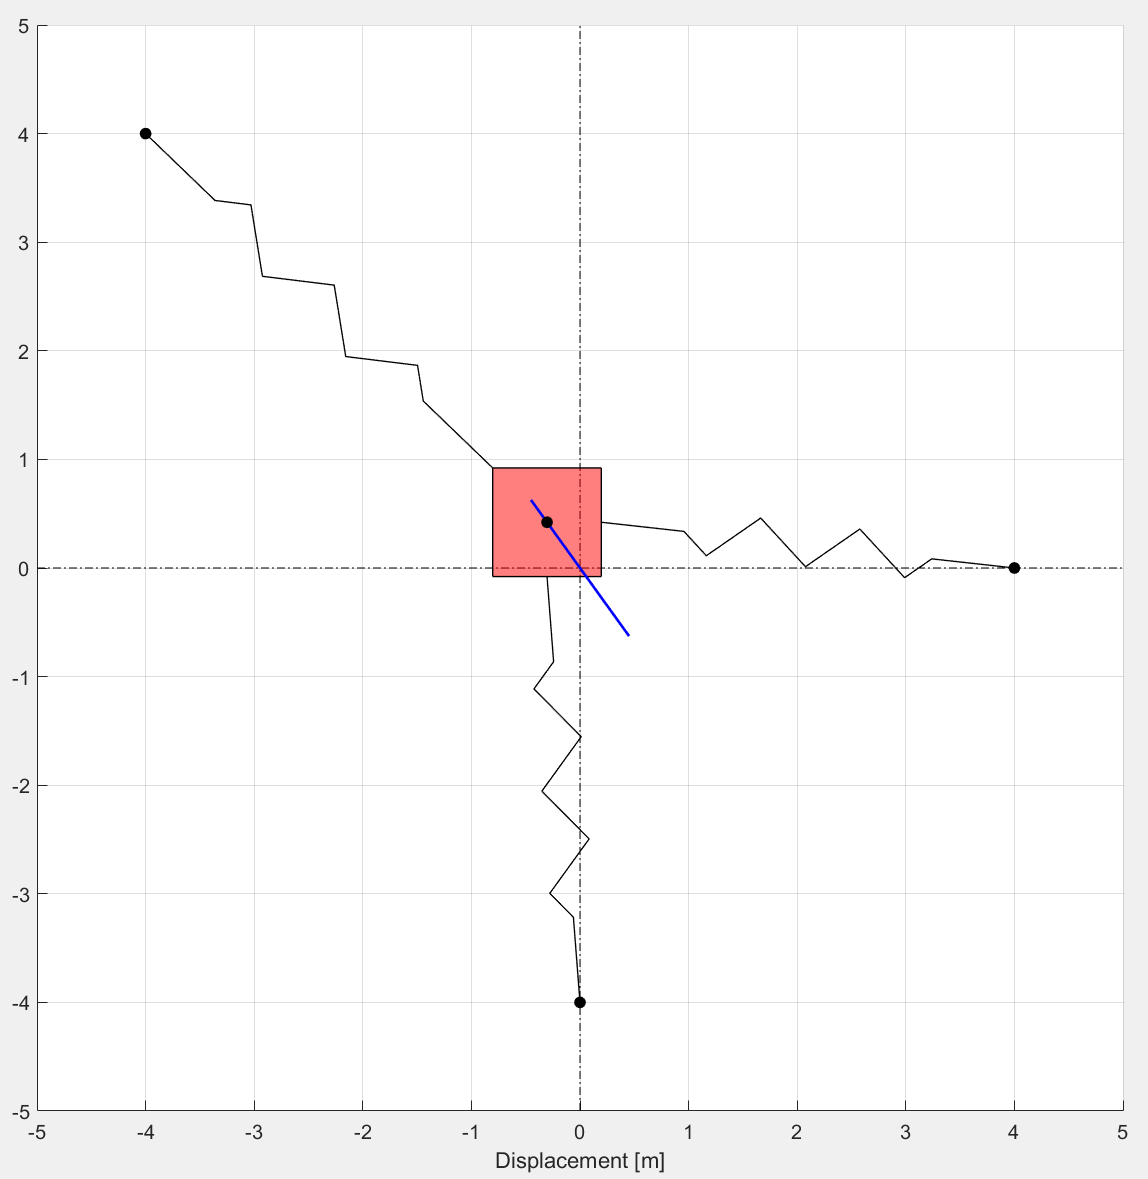
\includegraphics[width=0.9\linewidth]{mode1.png}
        \caption{Direction of First Mode}
        \label{fig:mode1}
    \end{subfigure}%
    \begin{subfigure}{.5\textwidth}
        \centering
        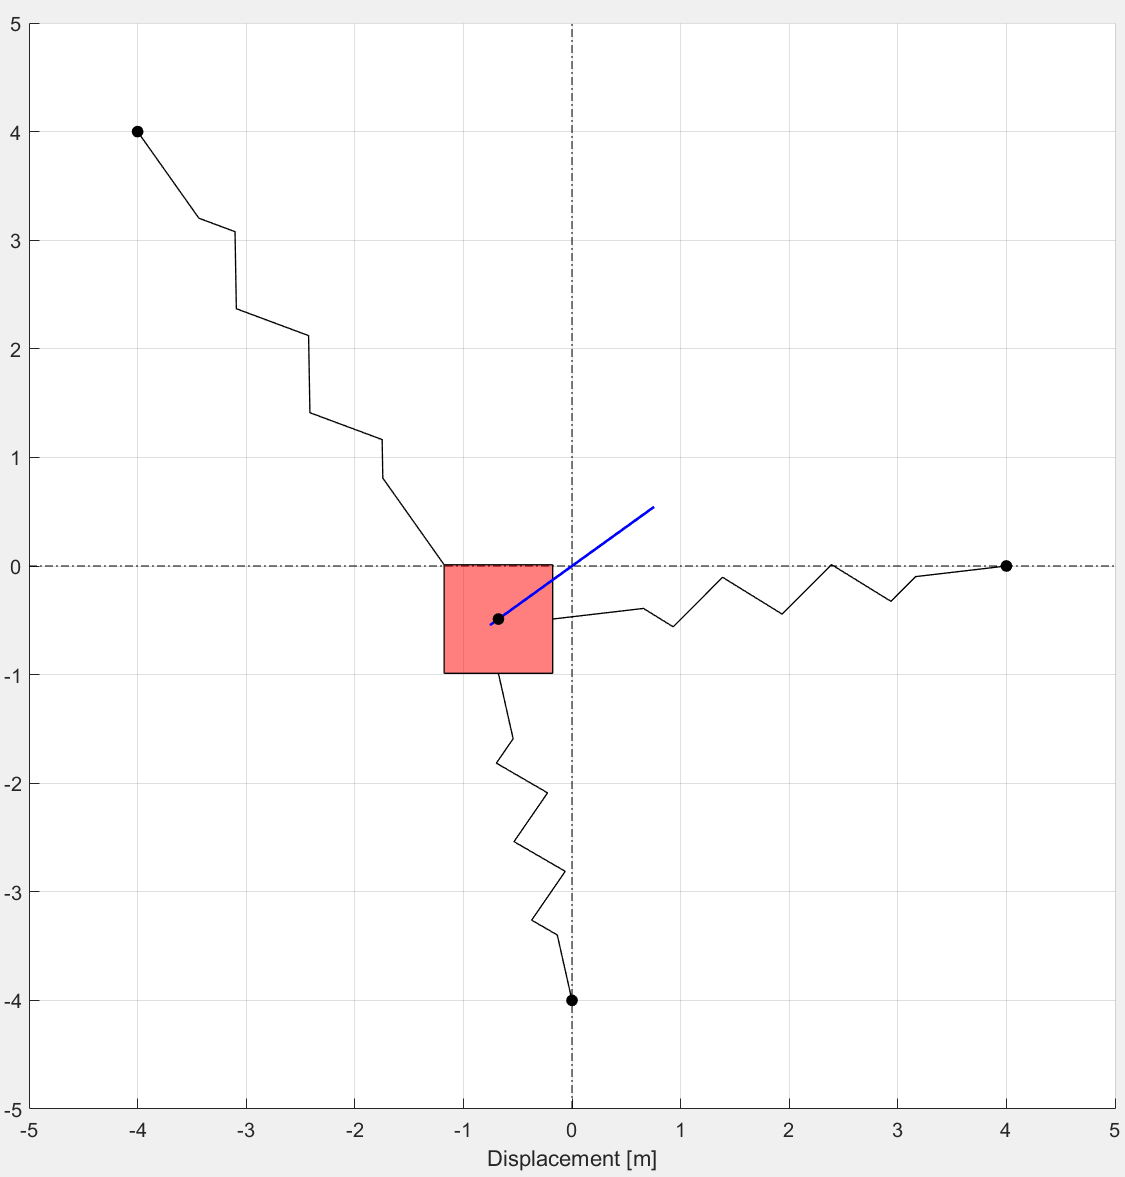
\includegraphics[width=0.9\linewidth]{mode2.png}
        \caption{Direction of Second Mode}
        \label{fig:mode2}
    \end{subfigure}
    
    \caption{System Modes}
\end{figure}

In order to excite the system along its mode, the eigenvectors corresponding to either eigenvalue pair can be plugged into the function as an initial state $x(0)$. It can be observed that the linear simulations do not match the nonlinear ones. This is due to the imprecision of the linearization operation performed; The farther the mass travels from the equilibrium point, the farther the nonlinear simulation diverges from the linear one. This is because the system matrices derived through linearization are only very accurate around the point about which they were linearized, that being the equilibrium point.

\paragraph{Natural Frequency}

\subsubsection{System Poles}

\paragraph{Example: System Poles}

\subsubsection{System Zeros}
The presence of a zero in an LTI system is an indication that the system can exhibit zero output even when the state and control input are nonzero. Intuitively: the presence of a zero implies that there are special combinations of non-zero initial conditions and non-zero control input that produce non-zero state time histories and zero output time histories.
\begin{equation*}
    x(0) \neq 0, u(t) \neq 0 \Rightarrow x(t) \neq 0, y(t) = 0
\end{equation*}
Components of the initial conditions and control input may combine and vanish, resulting in no perceptible contribution to the input. It follows that removing said components from the initial conditions and control input would generate the same output $y(t)$. \\
Not all LTI systems have zeros. Zeros are properties of the system at hand. Unlike poles, zeros do not influence the BIBO (\underline{\ref{sec:BIBO}}) stability of the system. The BIBO stability is determined by the location of its poles, even in cases that even have zeros in the right hald plane.

\paragraph{Formal Definition of a Zero}
Goal: find non-zero initial conditions and control input so that the output is zero for all time.
\begin{equation*}
    \zeta (t) := \begin{bmatrix}
        x(t) \\ u(t)
    \end{bmatrix} \neq 0 \Rightarrow y(t) = 0
\end{equation*}

\paragraph{Minimum Phase vs. Non-minimum Phase Zeros}
Minimum phase zeros are zeros that have non-positive real parts. Non-minimum phase zeros are zeros that have positive real parts. The naming convention follow from the Bode plot. If both are arranged symmetrically about the $i\omega$ axis, they will generate the same Bode magnitude plot, but the minimum phase plot will lie below that of the non-minimum phase plot. \\
To build intuition on the effect minimum and non-minimum phase zeros have on a system, consider an MSD system, with transfer function:
\begin{equation*}
    T(s) = \frac{Y(s)}{U(s)} = \frac{s \pm z}{s^2 + 2\zeta \omega_n s + \omega_n^2}
\end{equation*}
which exhibits two stable poles and one zero, which is a minimum if the + sign is used, and non-minimum if the - sign is used. We can rearrange the above equation and take its inverse Laplace transform to obtain a time-domain representation of the system.
\begin{equation*}
    \dot{u}(t) \pm zu(t) = f(t) = \ddot{y}(t) + 2\zeta\omega_n\dot{y}(t) + \omega_n^2
\end{equation*}
We have introduced $f(t)$ to represent the forcing function. In this representation we can understand the zeros as determining the input dynamics that relate the control input $u(t)$ to the forcing function $f(t)$. Likewise, the poles can be understood as determining the output dynamics that relate the forcing function $f(t)$ to $y(t)$.

\paragraph{Example: System Zero}
To demonstrate a system zero, take the example of a triple mass-spring-damper system, in which the input is the forcing applied to $m_1$. Defining the output as $p_2$, the input that results in a zero output (motion) in $m_2$ can be found.
\begin{figure}[H]
    \centering
    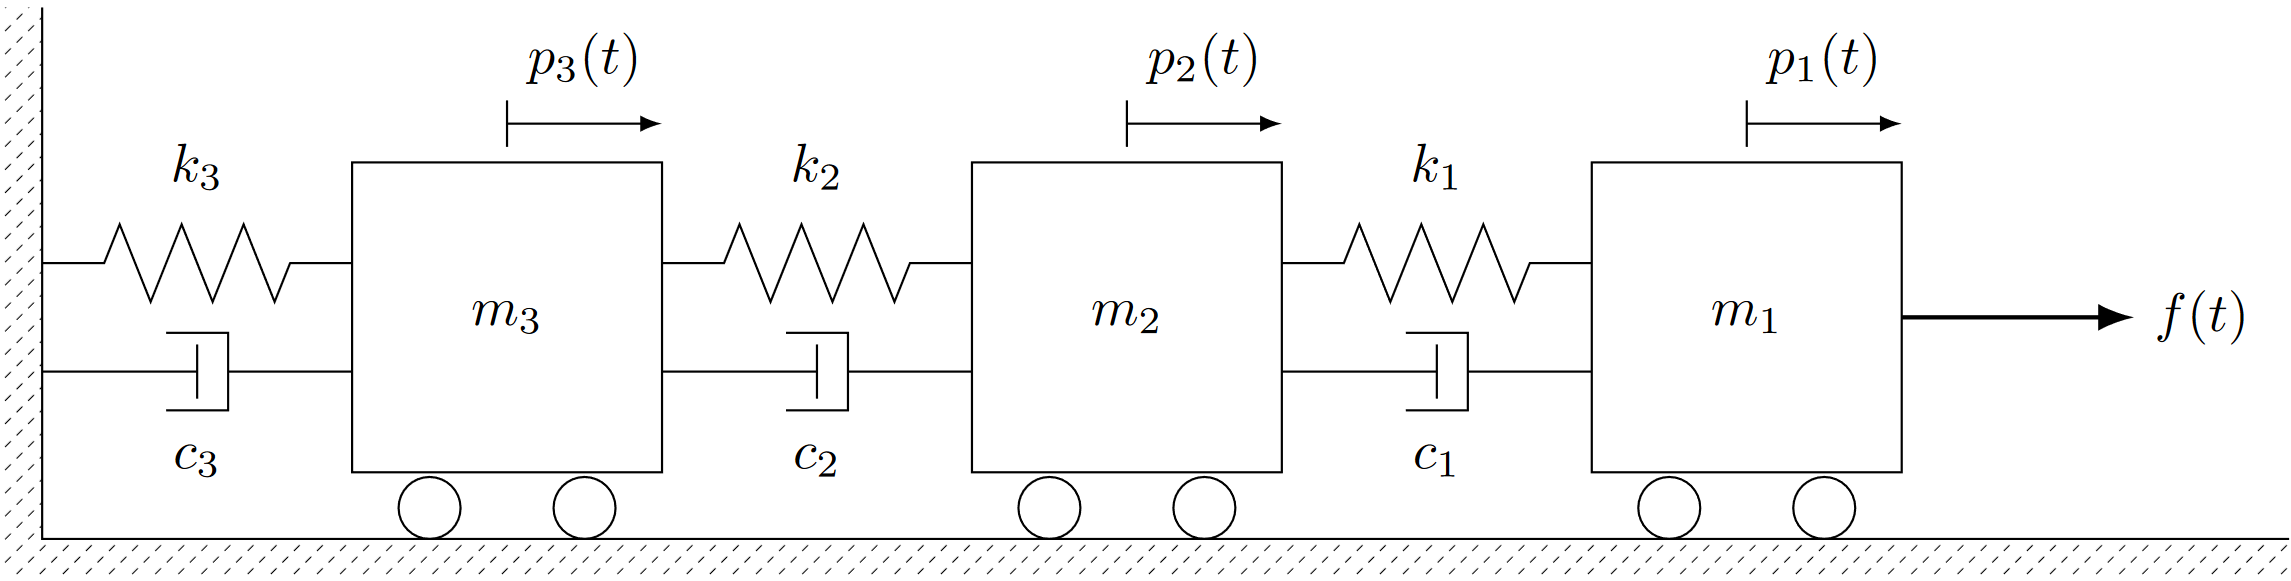
\includegraphics[width=1\linewidth]{3MSD.png}
    \caption{Triple Mass-Spring-Damper System}
    \label{fig:3MSD}
\end{figure}
The equations of motion (derived from Newton's laws) are as follows:
\begin{align*} 
    m_1 \ddot{p}_1(t) &= k_1(p_2(t) - p_1(t)) + c_1(\dot{p}_2(t) - \dot{p}_1(t)) + f(t) \\
    m_2 \ddot{p}_2(t) &= k_1(p_1(t) - p_2(t)) + k_2(p_3(t) - p_2(t)) + c_1(\dot{p}_1(t) - \dot{p}_2(t)) + c_2(\dot{p}_3(t) - \dot{p}_2(t)) \\
    m_3 \ddot{p}_3(t) &= k_2(p_2(t) - p_3(t)) - k_3p_3(t) + c_2(\dot{p}_2(t) - \dot{p}_3(t)] - c_3 \dot{p}_3(t)
\end{align*}
These equations of motion can then be arranged into the LTI state-space matrix form, giving the following state matrices.
\begin{equation*} 
  A =
  \begin{bmatrix}
    0 &0 &0 &1 &0 &0 \\
    0 &0 &0 &0 &1 &0 \\
    0 &0 &0 &0 &0 &1 \\
     -k_1/m_1 &k_1/m_1 &0 &- c_1/m_1 &c_1/m_1 &0 \\
     k_1/m_2 &- (k_1 + k_2)/m_2 &k_2/m_2 &c_1/m_2 &- (c_1 + c_2)/m_2 &c_2/m_2 \\
    0 &k_2 / m_3 &- (k_2 + k_3)/m_3 &0 &c_2/m_3 &- (c_2 + c_3)/m_3
  \end{bmatrix}
\end{equation*}

\begin{equation*}
    B =
    \begin{bmatrix}
        0 \\
        0 \\
        0 \\
        \frac{1}{m_1} \\
        0 \\
        0
    \end{bmatrix},
\quad
  C =
  \begin{bmatrix}
  0 &1 &0 &0 &0 &0
  \end{bmatrix},
  \quad
  D =
  \begin{bmatrix}
  0
  \end{bmatrix}
\end{equation*}
The system zeros can easily be found by converting the state space system into a zero-pole-gain form using MATLAB's \verb|zpk()| function. The poles of the system are compared to the zeros to establish which pole-zero pairs cancel, and which pole will lead to the desired system behavior. None of the zeros overlap a pole, yet the first zero has only a real component, indicating a lack of oscillation. The second and third zeros are conjugate pairs with only imaginary components. The second zero $ s_0 = 0 + 1.4142i $ was used for the following computations.

The initial condition vector was computed by setting up a generalized eigenvalue problem matrix using the system matrices.

\begin{equation*} \label{eq:eigenmatrix}
    A_z =
  \begin{bmatrix}
    s_0 I - A &-B  \\
    C &D 
  \end{bmatrix}
\end{equation*}

The null space of the $A_z$ matrix corresponds to the initial state $x_0$ and forcing input $u_0$. The values calculated for these variables is as follows:

\begin{equation*}
    x_0 = 
    \begin{bmatrix}
        -0.0098 \\
        0.0000 \\
        0.4964 \\
        -0.0973 \\ 
        0.0000 \\ 
        -0.0003
    \end{bmatrix},
    \quad
    u_0 = 
    \begin{bmatrix}
        -0.4768 - 0.1378i
    \end{bmatrix}
\end{equation*}

The system is then solved using MATLAB's \verb|ode45()| function. The initial state $x_0$ and input $u_0$ can be plugged into the system to confirm that $m_2$ demonstrates zero motion.

\subsubsection{System Modes for Second-order Systems}

\subsection{System Stability}
\subsubsection{Bounded Input, Bounded Output Stability} \label{sec:BIBO}
\subsubsection{Routh-Hourwitz Criterion}
\subsubsection{Nyquist Criterion}

\subsection{Sensitivity}
\subsubsection{Cosensitivity}

% \subsection{Frequency Domain Methods}


\end{document}